\documentclass{beamer}
\usetheme{CambridgeUS}

\usepackage{tikz}
\usetikzlibrary{calc,positioning}

\title{Stochastic Processes}
\author{Matteo Sani}
\begin{document}
\begin{frame}[plain]
    \maketitle
\end{frame}

%{
%\setbeamertemplate{background} 
%{\includegraphics[width=\paperwidth,height=\paperheight]{MyBackground.jpg}}

%\begin{frame}{Outline}
%	\begin{itemize}
%		\item Foundations
%		\begin{itemize}
%			\item Forward rate agreements and Forward rates: the devils is in the details
%			\begin{itemize}
%				\item A detailed proof of the FRA via the Expectation Operator
%			\end{itemize}
%		\end{itemize}
%		\item Interest rate swaps
%		\begin{itemize}
%			\item Basis swaps
%			\item Bonds and Swaps
%		\end{itemize}
%		\item Options in Interest Rates and the Black Model
%		\begin{itemize}
%			\item Caps and Floors
%			\item The valuation: the (ex) standard Black 76 model
%			\item Fixing Black Model: the shifted Lognormal Model
%			\item Swaptions
%			\item Bermudan Swaptions and Callable Bonds
%			\item How traders use Caps\&Floors and Swaptions in Practice
%		\end{itemize}
%	\end{itemize}
%\end{frame}

\begin{frame}{Outline}
	\tableofcontents
\end{frame}

\section{Random Variables}
\begin{frame}{Random Variables}
A variable whose value is a number determined by the outcome of a random experiment is called a \textcolor{red}{random variable}.
\newline

There are two kinds of random variable:
\begin{itemize}
	\item Discrete Random Variable
	\item Continuous Random Variable
\end{itemize}
\end{frame}

\subsection{Properties and Characteristics of Random Variables}
\begin{frame}{Discrete and Continuous Random Variables}
	\begin{block}{Discrete Random Variable} 
		If a random variable takes only a countable number (finite) of values, it is called discrete.
	\end{block}
	
	\small{
	\textbf{Example:} when 3 coins are tossed, the number of heads obtained is the random variable $X$, which assumes the values $\Omega=\{0,1,2,3\}$ ($\Omega$ ia a countable set).}
	\newline
	
	\begin{block}{Continuous Random Variable} 
		A random variable $X$ which can take any value between certain interval is called continuous.
	\end{block}
	
	\small{\textbf{Example:} the height of students in a particular class lies between 160 and 190~cm $(X = \{x|160 \leq x \leq 190\})$.}
	\begin{tikzpicture}[remember picture,overlay]
		\node[xshift=5cm,yshift=-3.7cm] (image) at (current page.center) {
\includegraphics[width=20px]{python_logo}};
		\node[align = center, yshift=1.45cm, below=of image] {\tiny{\href{shorturl.at/JR059}{shorturl.at/JR059}}};
	\end{tikzpicture}
\end{frame}

\begin{frame}{Probability Distribution}
Let $X$ be a random variable defined on a domain $\Omega$ of possible outcomes. 
\renewcommand{\arraystretch}{1.4}
\begin{table}[bt]
	\begin{tabular}{|c|c|} \hline
		\textbf{Discrete} & \textbf{Continuous} \\ \hline
		Probability Mass & Probability Density \\ \hline		
		\multicolumn{2}{|c|}{$f(x) = P(X=x)\;\forall x\in\Omega$}\\ \hline
		$P_i \geq 0;\;\forall i$ & $f(x) \geq 0;\;-\infty < x < \infty$\\ \hline
		$\sum_{i=0}^{n} P_i = 1$ & $\int_{-\infty}^{\infty} f(x) dx = 1$\\ \hline
		\multicolumn{2}{|c|}{Cumulative Distribution} \\ \hline
		$F(x) = P(X<x_i) = \sum_{x_i<x} P_i$ & $F(x) = P(X<a) = \int_{-\infty}^{a} f(x) dx$ \\ \hline
	\end{tabular}
\end{table}
\end{frame}

\begin{frame}{Characterizing a Random Variable}
	If we know the distribution of a random variable, we pretty much know all there is to know about it. 
	\newline
	\begin{columns}
		\column{0.45\linewidth}
		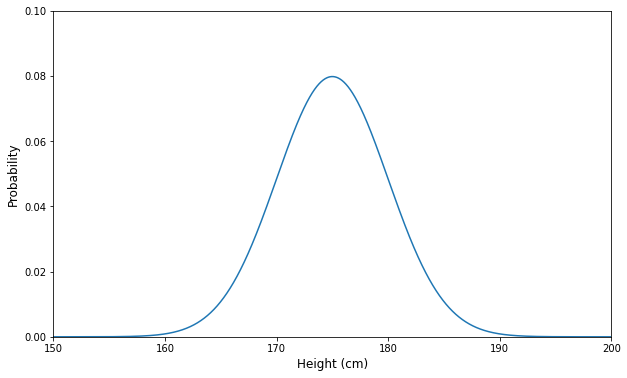
\includegraphics[height=3cm]{continouos_random_variable}
		\column{0.45\linewidth} 
		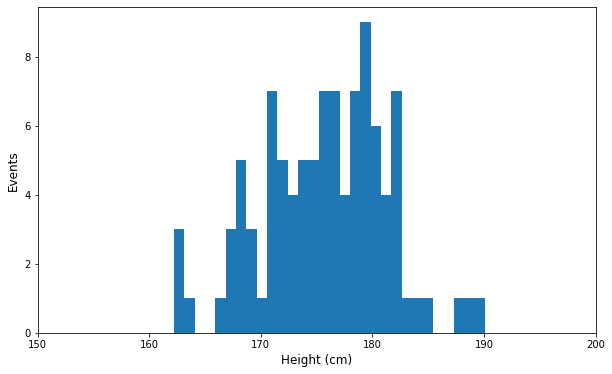
\includegraphics[height=3 cm]{real_data}
	\end{columns}

But with real data, we don't know the full distribution. So we want to characterize it by a couple of numbers (\emph{statistics}).
\footnotesize{
	\begin{itemize}
		\item mean, $\mu = \mathbb{E}[X] = \int_{-\infty}^{\infty} xf(x)dx$
		\item variance, 
		$\sigma^2 = \mathbb{E}[(X-\mu)^2] =\int_{-\infty}^{\infty} (x-\mu)^2f(x)dx$,
\end{itemize}}
\end{frame}

\subsection{Expectation and Its Properties}
\begin{frame}{Properties of Expectation}
	\renewcommand{\arraystretch}{1.4}
	\footnotesize{\tiny {\tiny }}{
	\begin{table}[bt]
		\begin{tabular}{|c|c|} \hline
Scalar multiplication & $\mathbb{E}[aX] = a\mathbb{E}[X]$ \\ \hline
Sums & $\mathbb{E}[X_1+\ldots X_K] =  \mathbb{E}[X_1] +\ldots + \mathbb{E}[X_n]$ \\ \hline
Linear combinations & $\mathbb{E}[a_1X_1+\ldots a_KX_K] =  a_1\mathbb{E}[X_1] +\ldots + a_K\mathbb{E}[X_K]$ \\ \hline
Expected value of a constant & $\mathbb{E}[a] = a$ \\ \hline
Products (independent variables) & $\mathbb{E}[XY] = \mathbb{E}[X] \mathbb{E}[Y]$ \\ \hline
		\end{tabular}
	\end{table}
}
\end{frame}

\section{Stochastic Processes}
\begin{frame}{Stochastic Process}
Real world data is noisy (i.e. distorted), and exhibits behaviours that cannot be described by a deterministic model (always produce same result from same inputs).
\newline

\begin{tabular}{cl}  
	\begin{tabular}{c}
		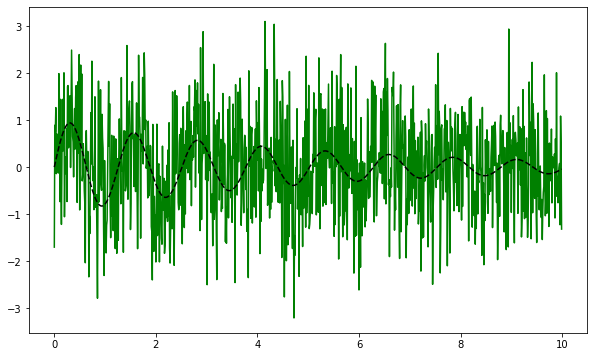
\includegraphics[height=3cm]{stochastic_process}
	\end{tabular}
	& \begin{tabular}{l}
		\parbox{0.45\linewidth}{
			Need to switch to \textcolor{red}{stochastic processes} in order to model the uncertainty of data.  
		}
	\end{tabular}  \\
\end{tabular}
\begin{block}{Stochastic process}
A collection of random variables that is indexed by some mathematical set (usually time).
\end{block}
\end{frame}

\subsection{SDE}
\begin{frame}{Stochastic Process}
	
Stochastic processes are described by \emph{stochastic differential equation} (SDE):

\begin{equation*}
\begin{aligned}
dX(t) = \mu(t,X(t)) dt &+ \sigma(t,X(t)) dW(t) \\  & =\underbrace{\mu(t,X(t))dt}_{\textrm{deterministic}} + \underbrace{\sigma(t,X(t)) \mathcal{N}(0,1)\sqrt{dt}}_{\textrm{stochastic}}
\end{aligned}
\end{equation*}

\begin{tabular}{cl}  
	\begin{tabular}{c}
		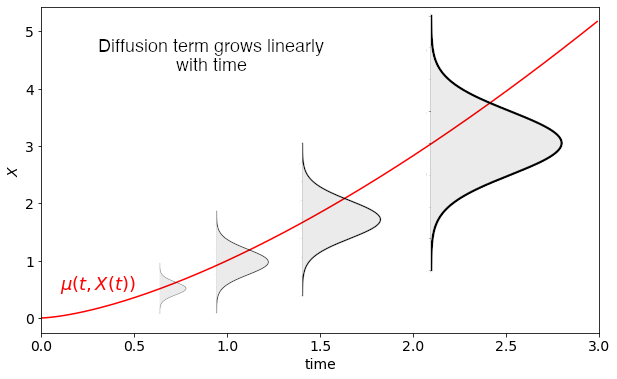
\includegraphics[height=3.2cm]{brownian_process}
	\end{tabular}
	& \begin{tabular}{l}
		\parbox{0.45\linewidth}{
			\begin{itemize}
				\item The mean of $dW$ is zero and its variance is $dt$
				\item the standard deviation grows with the square root of time: $W(t) \simeq \mathcal{N}(0, t)$ because each $dW$ is distributed like independent standard Gaussian.
			\end{itemize}  
		}
	\end{tabular}  \\
\end{tabular}
\end{frame}

\subsection{Martingales}
\begin{frame}{Martingale}
\begin{block}{Definition}
A \textcolor{red}{martingale} is a (integrable and adapted) stochastic process which models a fair game with the following remarkable feature
\begin{equation}
\mathbb{E}[X_t|\mathcal{F}_s] = X_s
\end{equation}
so the best prediction for the future value $X_t$, given the knowledge $\mathcal{F}_s$ at time $s$ is the value at time $s$ itself, $X_s$.
\end{block}
\end{frame}

\subsection{Martingales}
\begin{frame}{Martingale}
	\begin{block}{Properties}
		If $X_t$ is a stochastic process with volatility $\sigma_t$, which satisfies $\mathbb{E}[(\int_0^T\sigma^2_s ds)^{\frac{1}{2}}]<\infty$, and SDE $dX_t=\sigma_t dW_t+\mu_t dt$ 
		\begin{equation*}
			X\text{ is a martingale } \iff X\text{ is drift-less } (\mu_t=0)
		\end{equation*}
	\end{block}	
A martingale corresponds to the common notion that "an efficient price, changes randomly" so we cannot know if it will go up or down. That is why this mathematical concept is brought into finance.

	\begin{tikzpicture}[remember picture,overlay]
		\node[xshift=-5cm,yshift=-3.7cm] (image) at (current page.center) {
\includegraphics[width=20px]{python_logo}};
		\node[align = center, yshift=1.45cm, below=of image] {\tiny{\href{shorturl.at/knyGT}{shorturl.at/knyGT}}};
	\end{tikzpicture}
\end{frame}

\subsection{Geometric Brownian Motion (GBM)}
\begin{frame}{Geometric Brownian Motion}
\begin{itemize}
	\item Trade random fluctuations deviate a stock price $S_t$ from a steady state.
	\item The price relative change in $dt$ can be decomposed into two parts
	\begin{itemize}
		\item \emph{deterministic}: the expected return from holding the stock during $dt$. It can be expressed as $\mu S_tdt$ (with $\mu$ being the expected rate of return);
		\item \emph{stochastic}: model the random changes of the market. A reasonable assumption is to equal this term to $\sigma S_t dW_t$. 
	\end{itemize}
	\item Putting all together, the resulting SDE is
	\begin{equation}
		\begin{gathered}
		dS_t = \mu S_t dt + \sigma S_t dW_t \\
		\frac{dS_t}{S_t} = d\log(S_t) = \mu dt + \sigma dW_t
		\end{gathered}
		\label{eq:log_normal_sde}
	\end{equation}
\end{itemize}
\end{frame}

\subsubsection{Ito's Lemma}
\begin{frame}{Ito's Lemma}
	\begin{block}{Ito's Lemma}
	For any given continuous and differentiable function $G(S,t)$ where S satisfies $dS=adt + bdW_t$, holds
	\begin{equation}
	dG = \left(a\frac{\partial G}{\partial S} + \frac{\partial G}{\partial t} + \underbrace{\frac{1}{2}b^2\frac{\partial^2 G}{\partial S^2}}_{\text{additional term}}\right)dt + b\frac{\partial G}{\partial S} dW
	\label{eq:itos_lemma}
	\end{equation}
	\end{block}

	This is essentially an extension of the \emph{Taylor series} for stochastic functions, in the expansion an extra ($2^{nd}$ order) term appears.
\end{frame}

\begin{frame}{Geometric Brownian Motion}
	\begin{itemize}
		\item So setting $G=\log(S_t)$ 
		\begin{equation*}
			\frac{\partial G}{\partial S}=\frac{1}{S_t},\;\frac{\partial G}{\partial t}=0,\;\frac{\partial^2 G}{\partial S^2}=-\frac{1}{S_t^2}
		\end{equation*}
		\item Substituting back into Ito's lemma Eq.~\ref{eq:itos_lemma} and taking $a$ and $b$ values from Eq.~\ref{eq:log_normal_sde}
		\begin{equation}
			\begin{gathered}
			d(\log S_t) = \left(\mu S_t\frac{1}{S_t} + \frac{1}{2}\sigma^2S_t^2\left(-\frac{1}{S_t^2}\right)\right)dt + \sigma dW \\
			\log(S_t) - \log(S_{t-1}) = \log\frac{S_t}{S_{t-1}}=\left(\mu - \frac{1}{2}\sigma^2\right)dt + \sigma dW \\
			S_t = S_{t-1}\exp\left[\left(\mu-\frac{1}{2}\sigma^2\right)dt + \sigma\mathcal{N}(0,1)\sqrt{dt}\right] 
			\end{gathered}
		\end{equation}
	\end{itemize}
\end{frame}

\subsubsection{Log-normality}
\begin{frame}{Log-normality}
\begin{itemize}
	\item The variation in $\log(S_t)$ equals a constant (the \emph{drift} $\mu-\frac{1}{2}\sigma^2$) plus a Gaussian distributed random variable. Therefore at some time $t$
	\begin{equation*}
		\log S_t = \mathcal{N}\left[\left(\mu -\frac{\sigma^2}{2}\right)t, \sigma^2 t\right]
	\end{equation*}
\end{itemize}
\begin{block}{Log-normal Variable}
A random variable whose logarithm is normally distributed is said to be \textcolor{red}{log-normal}.

One of the most important properties of a log-normal distribution is to be positive definite (a good characteristic for stock prices).
\end{block}
\begin{tikzpicture}[remember picture,overlay]
	\node[xshift=5cm,yshift=-3.7cm] (image) at (current page.center) {
\includegraphics[width=20px]{python_logo}};
	\node[align = center, yshift=1.45cm, below=of image] {\tiny{\href{shorturl.at/jovCST}{shorturl.at/jovCS}}};
\end{tikzpicture}
\end{frame}

\end{document}




